\documentclass[10pt, twoside]{article}
\usepackage{be-my-concrete, be-my-geometry}
\usepackage{extra-algebra}
\setcounter{MaxMatrixCols}{15}

\begin{document}

\pagestyle{empty}
\begin{abstract}
    А помните алгебру? Числа там, дроби всякие, уравнения, неравенства.
    На самом деле, это все ерунда. Алгебра -- про структуры, про симметрии.
    Этот курс именно про это, мы будет изучать, что называют ,,абстрактной`` алгеброй.
    Может вы слышали, как учитель на уроке случайно сказал, о поле действительных чисел, а не о множестве.
    А про целые числа, так он почему-то не говорил.
    Мы подвигаем разные фигурки, повертим бусы в руках. 
    
    Чтобы понять каждую тему, нужно иметь базовые знания про числа, операции с ними и многочлены.
    Также он подойдет для тех, кто не боится непонятных слов (например, группа преобразований,
    гомоморфизм и поле) и хочет разобраться в том, что они значат.
\end{abstract}

\newpage

\tableofcontents
\newpage

\setcounter{page}{1}
\pagestyle{fancy}

Алгебра -- наука о структурах, которые описываются с помощью операций и законов. 
Возможно, то что мы будем называть ,,алгебра`` -- это не совсем то, что вы привыкли называть ,,алгебра`` 
Потому что в школьном курсе алгебры, особенно в старших классах, почему-то изучается анализ, а не сама алгебра.

Первая структура, с которой мы с вами познакомимся -- это группы.
Это одно из самых ,,базовых понятий``, но оно же и является центральным. 

% --------------    1
\section{Перестановки}

Самая интерпретируемая группа -- это группа перестановок.
Вероятно, вы уже слышали о том, что такое перестановка, не задумываясь о её групповой структуре.
Для начала, ``нестрого'' разберемся с перестановками.

\begin{practice}
    Сколько есть способов переставить $n$ человек в очереди?
\end{practice}

\begin{example}
    Напишем, какое-нибудь слово, например: \[
        \text{\textsf{УШКА}}\footnote{Это слово осмысленное,
        но в дальнейшем, мы будем называть ``словами'' любые цепочки букв,
    не заботясь о том, являются ли они словами русского языка.}
    \] 
    За один шаг разрешается поменять местами любые две буквы.
    Например, можно поменяв буквы \textsf{А} и \textsf{К}, получить слово \[
        \text{\textsf{УШАК}}
    \] 
\end{example}

\begin{practice}
    Можно ли получить слово \textsf{КАШУ} из слова \textsf{УШКА} за один шаг?
    Если нет, то за какое минимальное число шагов можно это сделать?
\end{practice}

\begin{practice}\label{prac:word}
    Можно ли, начав, со слова \textsf{ТАПОК}, вернуться в исходное слово после 10 шагов?
    После 11 шагов?
\end{practice}

В \cref{prac:word}, вы заметили, что за 10 шагов все получилось. А вот за 11 -- никак.
На самом деле это не случайность, и верен более общий факт. 
\begin{proposition}
    Если на каждом шаге разрешено поменять только две буквы, 
    то за нечетное число шагов не получится вернуться в исходное слово.
\end{proposition}

Теперь возьмём другое слово, допустим, \textsf{АДО}. Есть три пары букв, которые можно поменять.
Так что, за один шаг мы можем получить три слова. 
\[
    \text{\textsf{ОДА}} \qquad \text{\textsf{ДАО}} \qquad \text{\textsf{АОД}}
\]
На втором шаге мы должны выбрать одно из этих слов и поменять в нём две буквы. 
Пару для обмена в каждом слове можно выбрать двумя способами, 
а два другие дадут новые слова. 
\begin{align*}
    \text{\textsf{ОДА}} &\to \text{\textsf{ДОА ОАД АДО}} \\
    \text{\textsf{ДАО}} &\to \text{\textsf{ДОА ОАД АДО}}\\
    \text{\textsf{АОД}} &\to \text{\textsf{ДОА ОАД АДО}}
\end{align*}
Видно, что в результате получаются одни и те же три слова.
\[
    \text{\textsf{ДОА}} \qquad \text{\textsf{ОАД}} \qquad \text{\textsf{АДО}}
\] 
\begin{practice}
    Проверьте, что за три шага получается тот же набор слов, что и за 1 шаг.
\end{practice}
Видно, что мы разбили все варианты на две группы по три слова
и на каждом шаге переходим из одной группу в другую: \[
    \text{\textsf{АДО ОАД ДОА}} \leftrightarrow \text{\textsf{ДАО АОД ОДА}}
\] 
А значит, вернуться в исходную группу (в частности, получить слово \textsf{АДО})
можно только за четное число шагов.

\subsection{Нотация перестановок}
\begin{definition}
    [Перестановка]
    Перестановка -- это функция, которая отображает множество букв в себя.
    \[
        \sigma: \{1, 2, \ldots, n\} \to \{1, 2, \ldots, n\}.
    \]
    
    Перестановка $\sigma$ может быть записана в виде\footnote{
    Существуют и другая запись: $(\sigma(1) \; \sigma(2) \; \sigma(3) \; \ldots \; \sigma(n))$.} \[
        \sigma = \begin{pmatrix}
            1 & 2 & 3 & \ldots & n \\
            \sigma(1) & \sigma(2) & \sigma(3) & \ldots & \sigma(n)
        \end{pmatrix}.
    \]
\end{definition}
\begin{example}
    При перестановка $\sigma = \begin{pmatrix}
        1 & 2 & 3 & 4 \\
        2 & 1 & 4 & 3
    \end{pmatrix}$ 
    Первая буква переходит на вторую, вторая -- на первую, третья -- на четвёртую, четвёртая -- на третью.
    Допустим, со словом \textsf{РЫБА} наша перестановка сделает (на \cref{fig:permutation}):
    \[
        \sigma(\text{\textsf{РЫБА}}) = \text{\textsf{ЫРАБ}}.
    \]

    \begin{figure}[ht]
        \centering
        \begin{asy}
            size(7cm);
            defaultpen(fontsize(10));

            pair[] start = {(0,0), (1,0), (2,0), (3,0)};
            string[] startText = {"Р","Ы","Б","А"};

            pair[] end = {(0,-2), (1,-2), (2,-2), (3,-2)};
            string[] endText = {"Ы","Р","А","Б"};

            // Подписи букв
            for(int i = 0; i < 4; ++i) {
                label(startText[i], start[i], N);
                label(endText[i], end[i], S);
            }

            // Кривые "ниточки"
            draw(start[0]..(0.3, -0.5)..end[1], blue+linewidth(1)); // Р -> Ы
            draw(start[1]..(0.6, -0.5)..end[0], blue+linewidth(1)); // Ы -> Р
            draw(start[2]..(2.4, -1.4)..end[3], longdashed+red+linewidth(1)); // Б -> А
            draw(start[3]..(2.8, -1.4)..end[2], longdashed+red+linewidth(1)); // А -> Б

            
        label("$\begin{pmatrix} 2 & 2 & 3 & 4 \\ 2 & 1 & 4 & 3 \end{pmatrix}$", (4.5, -1));
        \end{asy}
        \caption{Перестановка $\sigma$.}
        \label{fig:permutation}
    \end{figure}
\end{example}

\setcounter{footnote}{0}
Применяя одну перестановку за другой, мы можем получить новую перестановку. 
Для этого тоже есть запись. Пусть у нас есть две перестановки $\sigma$ и $\tau$.
Тогда их произведение $\sigma \circ \tau$ -- это перестановка, которая получается из $\tau$,
после чего к ней применяют $\sigma$\footnote{Да! Именно так! Слева-направо!}. 

\begin{example}
    Пусть $\sigma = \begin{pmatrix}
        1 & 2 & 3 & 4 \\
        2 & 1 & 4 & 3
    \end{pmatrix}$ и $\tau = \begin{pmatrix}
        1 & 2 & 3 & 4 \\
        2 & 4 & 3 & 1
    \end{pmatrix}$.
    Тогда их произведение будет равно: 
    \[
        \sigma \circ \tau = \begin{pmatrix}
            1 & 2 & 3 & 4 \\
            \sigma(\tau(1)) & \sigma(\tau(2)) & \sigma(\tau(3)) & \sigma(\tau(4))
        \end{pmatrix} = \begin{pmatrix}
            1 & 2 & 3 & 4 \\
            1 & 3 & 4 & 2
        \end{pmatrix}.
    \]
    
    Давайте рассмотрим, что у нас происходит на примере слова \textsf{КИНО} (на \cref{fig:permutation2}).
    
    \begin{figure}[h]
        \centering
        \begin{asy}
            size(7cm);
            defaultpen(fontsize(10));

            pair[] start = {(0,0), (1,0), (2,0), (3,0)};
            string[] startText = {"К","И","Н","О"};
            pair[] mid = {(0, -2), (1, -2), (2, -2), (3, -2)};
            string[] midText = {"О","К","Н","И"};
            pair[] end = {(0, -4), (1, -4), (2, -4), (3, -4)};
            string[] endText = {"К","О","И","Н"};

            for(int i = 0; i < 4; ++i) {
                label(startText[i], start[i], N);
                label(midText[i], mid[i], N);
                label(endText[i], end[i], S);
            }

            // Кривые "ниточки"
            draw(start[0]{(1, -1)}..(mid[1]+(0, 0.3)), blue+linewidth(1)); // К -> Н
            draw(start[1]{(1, -2)}..(mid[3]+(0, 0.3)), blue+linewidth(1)); // И -> О
            draw(start[2]..(mid[2]+(0, 0.3)), blue+linewidth(1)); // Н -> К
            draw(start[3]{(-6, -1)}..(mid[0]+(0, 0.3)), blue+linewidth(1)); // О -> И

            draw(mid[0]{(0.5, -2)}..end[1], longdashed+red+linewidth(1)); // Н -> О
            draw(mid[1]{(1, -2)}..end[0], longdashed+red+linewidth(1)); // О -> Н
            draw(mid[2]{(3, -2)}..end[3], longdashed+red+linewidth(1)); // К -> И
            draw(mid[3]{(-5, -2)}..end[2], longdashed+red+linewidth(1)); // И -> К

            label(scale(0.9)*"$\begin{pmatrix} 1 & 2 & 3 & 4 \\ 2 & 4 & 3 & 1 \end{pmatrix}$", (4.5, -0.7));
            label(scale(0.9)*"$\begin{pmatrix} 1 & 2 & 3 & 4 \\ 2 & 1 & 4 & 3 \end{pmatrix}$", (4.5, -2.7));
            
        \end{asy}
        \caption{Перестановка $\sigma \circ \tau$.}
        \label{fig:permutation2}
    \end{figure}
\end{example}

\begin{practice}
    Найдите композицию $\tau \circ \sigma$. Проверьте, что это не то же самое, что $\sigma \circ \tau$.
\end{practice}

\begin{definition}
    [Циклическая запись]
    Любую перестановку можно записать в виде произведения циклов.
    Например, перестановка $\sigma$ (на \cref{fig:permutation4}) \[
        \sigma = \begin{pmatrix}
            1 & 2 & 3 & 4 & 5 & 6 \\
            3 & 1 & 5 & 6 & 2 & 4
        \end{pmatrix}.
    \] 
    Записывается в виде: \[
        \sigma = |1 \; 3 \; 5 \; 2\rangle |4 \; 6\rangle.
    \]
    У такой записи есть ``свобода выбора''. Один и тот же цикл можно записать по-разному. 
    Например, \[
        |1 \; 3 \; 5 \; 2\rangle = |3 \; 5 \; 2 \; 1\rangle = |5 \; 2 \; 1 \; 3\rangle = |2 \; 1 \; 3 \; 5\rangle.
    \]

    Мы будем говорить, что у перестановки $\sigma$ цикловой тип $\left( 4,2 \right)$ 
    (в данном случае, это значит, что у нас есть один 4-цикл и один 2-цикл).
    А иногда еще будем рисовать диаграмму Юнга (на \cref{fig:permutation3}), данного циклового типа.

    \begin{figure}[ht]
        \centering
        \begin{asy}
            size(2cm);
            defaultpen(fontsize(10));

            draw(unitsquare);
            draw(shift(1, 0)*unitsquare);
            for (int i = 0; i < 4; ++i) {
                draw(shift(i, 1)*unitsquare);
            }
                

            label("1", (0.5, 1.5));
            label("3", (1.5, 1.5));
            label("5", (2.5, 1.5));
            label("2", (3.5, 1.5));
            label("4", (0.5, 0.5));
            label("6", (1.5, 0.5));
        \end{asy}
        \hspace{1cm} или просто \hspace{1cm}
        \begin{asy}
            size(2cm);
            defaultpen(fontsize(10));

            draw(unitsquare);
            draw(shift(1, 0)*unitsquare);
            for (int i = 0; i < 4; ++i) {
                draw(shift(i, 1)*unitsquare);
            }
        \end{asy}
        \caption{Цикловой тип перестановки $\sigma$.}
        \label{fig:permutation3}
    \end{figure}

\end{definition}
\begin{figure}[ht]
    \centering
    \begin{asy}
        size(7cm);
        defaultpen(fontsize(10));

        pair[] start = {(0,0), (1,0), (2,0), (3,0), (4,0), (5,0)};
        string[] startText = {"1","2","3","4","5","6"};
        pair[] end = {(0,-2), (1,-2), (2,-2), (3,-2), (4,-2), (5,-2)};
        string[] endText = {"3","1","5","6","2","4"};
        // Подписи букв
        for(int i = 0; i < 6; ++i) {
            label(startText[i], start[i], N);
            label(endText[i], end[i], S);
        }

        // Кривые "ниточки"
        draw(start[0]{(1, -2)}..end[2], blue+linewidth(1)); // 1 -> 3
        draw(start[1]{(1.2, -2)}..end[4], blue+linewidth(1)); // 2 -> 5
        draw(start[2]{(1, -2)}..end[1], blue+linewidth(1)); // 3 -> 1
        draw(start[3]{(6, -1)}..end[5], longdashed+red+linewidth(1)); // 4 -> 6
        draw(start[4]{(-3, -1)}..end[0], blue+linewidth(1)); // 5 -> 2
        draw(start[5]{(-3, -2)}..end[3], longdashed+red+linewidth(1)); // 6 -> 4

        label(scale(0.8)*"$\begin{pmatrix} 1 & 2 & 3 & 4 & 5 & 6 \\ 3 & 1 & 5 & 6 & 2 & 4 \end{pmatrix}$", (8, -1));
    \end{asy}
    \caption{Циклическая запись перестановки.}
    \label{fig:permutation4}
\end{figure}

Есть одно важное понятие, которое может таким не показаться.
Возможно, мы не сможем в полном объеме раскрыть его в этом курсе, но что же поделать.
Перед этим, скажем, что \emph{транспозиция} -- это перестановка, которая меняет местами только две буквы.

\begin{definition}
    [Четность перестановки]
    Перестановка называется четной, если она может быть записана в виде произведения четного числа транспозиций.
    Иначе, она называется нечетной.
\end{definition}

\begin{definition}
    [Порядок перестановки]
    Порядок перестановки $\sigma$ -- это наименьшее число $n$, такое что \[
        \sigma^n = \text{id}.
    \]
\end{definition}

\begin{theorem}
    [Порядок перестановки]
    Порядок перестановки $\sigma$ равен наибольшему общему делителю длин всех циклов в её циклической записи.
\end{theorem}
\begin{proof}
    Цикл длины $k_i$ возвращает элементы на место после $k_i$ применений. Поскольку циклы не пересекаются, порядок всей перестановки — минимальное число $k$, при котором $k$ делится на каждое $k_i$.  
    Это и есть наименьшее общее кратное $k_1, k_2, \dots, k_m$.
\end{proof}

% --------------    2
\section{Введение в группы}

\epigraph{Симметрия, как бы широко или узко мы не понимали это слово, есть идея, с помощью которой человек веками пытался объяснить и создать порядок, красоту и совершенство.}{Герман Вейль.}

<<Теория групп>> расшифрует и формализует понятие \emph{симметрии}. Например, когда мы говорим, что у человека симметричное лицо, мы подразумеваем, что мы можем отразить его лицо относительно \emph{оси симметрии}, и оно будет выглядить абсолютно также. Это утверждение о действии. Или, например, снежинка тоже симметрична, но во много большем порядке: мы можем поворачивать ее на $60^\circ$ или на $120^\circ$, можно отражать ее относительно множества осей симметрии или не делать ничего; и все эти преобразования оставят ее вид прежним. Вот такое вот собрание действий и называется группой. 

Вернее, если бы более чеcтным, то группа это более формальное и абстрактное понятие. Например, как и число 3. Обращаясь к нему мы не задумываемся о каком именном числе объектов идет речь: не важно головки сыра это или миллиарды лет. Но с числом работать намного удобнее: складывая два числа, мы совсем-совсем уже забываем о изначальной ,,природе``.
\subsection{Определение группы}
\begin{definition}
    [Группа]
    Это множество $G$ с операцией $\star$, которое обладает следующими свойствами: 
    \begin{conditions}
        \item \textit{Замкнутость}: $$\forall a, b \in G: a \star b \in G.$$
        \item \textit{Ассоциативность}: $$\forall a, b, c \in G: (a \star b) \star c = a \star (b \star c).$$
        \item \textit{Наличие нейтрального элемента}: $$\exists e \in G: \forall a \in G: e \star a = a.$$
        \item \textit{Наличие обратного элемента}: $$\forall a \in G: \exists a^{-1} \in G: a \star a^{-1} = e.$$
    \end{conditions}
    Для группы также существует обозначение: $(G, \star).$
    Если группа $G$ конечна, то ее порядок $|G|$ -- это количество элементов в ней.
\end{definition}

Стоит еще обратить свое внимание на то, насколько общеупотребимое слово выбрано для этого понятия, для казалось бы, такого спицифического объекта симметрий. Это показатель фундаментальности и общности этого понятия.
Группа фиксирует суть симметрии объекта --- не сами движения, а то, как они сочетаются друг с другом. Операция в группе (композиция) кодирует вопрос: 'Если я сделаю преобразование A, а потом преобразование B, какое одно преобразование C даст тот же итоговый эффект?' Именно эта структура (замкнутость, ассоциативность, наличие 'ничего' и 'отмены') делает группы универсальным инструментом для описания симметрий любой природы.

Существуют различные классификации групп. Например, классификация по типу операции. 
Бывают группы по сложению (аддитивные), то есть с операцией сложения. 
А также бывают группы по умножению (мультипликативные) -- с операцией умножения.


\begin{example}
    Группа отражений лица по вертикали называется группой $\Z/(2)$ и состоит ровно из двух элементов: ничего не делать и сделать что-то.
\end{example}
\begin{example}
        $(\Z, +)$ множество целых чисел с операцией сложения.
\end{example}
\begin{example}
    $({\Z}/{(5)}, +)$ множество остатков по модулю 5 с операцией сложения.
\end{example}
\begin{example}
    $(R, \cdot)$ множество действительных чисел с операцией умножения.
\end{example}
\begin{example}
    Как множество -- движения правильной фигуры, а операция тут -- композиция этих движений.
    Например, у нас есть квадрат. Мы можем его поворачивать на 90 градусов,
    а также можем его отражать относительно осей симметрии.
    Тогда у нас получится группа, которая называется $D_4$\footnote{
    Также такую группу можно было назвать $\mathrm{Isom}(\square) $.}, 
    она состоит из 8 элементов (на \cref{fig:group}):

    \begin{multicols}{2}
        \begin{itemize} 
            \item $e$ --- ничего не делать;
            \item $r$ --- поворот на 90 градусов;
            \item $r^2$ --- поворот на 180 градусов;
            \item $r^3$ --- поворот на 270 градусов;
            \item $s_1$ --- отражение относительно оси симметрии по оси $x$;
            \item $s_2$ --- отражение относительно оси симметрии по оси $y$;
            \item $s_3$ --- отражение относительно диагонали, которая идет из левого верхнего угла в правый нижний;
            \item $s_4$ --- отражение относительно диагонали, которая идет из правого верхнего угла в левый нижний.
        \end{itemize}
    \end{multicols}
\end{example}

\begin{figure}[h]
    \centering
    \begin{asy}
        size(5cm);
        draw((0,0)--(1,0)--(1,1)--(0,1)--cycle, linewidth(bp));
        draw((0.5,-0.1)--(0.5,1.1), dashed+blue);
        draw((-0.1,0.5)--(1.1,0.5), dashed+blue);
        draw((-0.1, -0.1)--(1.1, 1.1), dashed+blue);
        draw((1.1, -0.1)--(-0.1, 1.1), dashed+blue);
        label("$s_1$", (0.5,-0.2), blue);
        label("$s_2$", (-0.2, 0.5), blue);
        label("$s_4$", (1.2, 1), blue);
        label("$s_3$", (-0.2, 1), blue);
        draw("$r$", (1.1,0.3){right}..{left}(1.1,0.7), red, arrow=Arrow(TeXHead));
    \end{asy}
    \caption{Группа движений квадрата}
    \label{fig:group}
\end{figure}

\begin{example}[Симметрическая группа]
    До этого мы рассматривали с вами перестановки букв в словах.
    Такие перестановки тоже образуют группу. Она обозначается $S_n$, 
    где $n$ --- количество букв в слове, а называется \emph{симметрической}.
\end{example}

\begin{example}[Группа кубика Рубика]
    Примером группы огромного порядка ($\sim 4,3\cdot 10^{19}$) может быть группа кубика Рубика. Повороты граней кубика Рубика образуют группу. Композиция поворотов --- это наша операция. 'Ничего не делать' --- нейтральный элемент. Обратный элемент --- поворот в обратную сторону или последовательность ходов, отменяющая действие. Эта группа не коммутативна: повернуть верхнюю грань, а потом правую --- не то же самое, что повернуть правую, а потом верхнюю!
\end{example}

\begin{example}[Группа автоморфизмов множества]\label{ex:AutX}
Все взаимно однозначные отображения множества $X$ в себя (перестановки его элементов) образуют группу. Она обозначается $\Aut X$ и называется \emph{группой автоморфизмов} множества $X$. Если группа $X$ конечна, то $\Aut X \cong S_{|X|}$.
\end{example}

Заострим свое внимание на том, насколько важна структура, которую мы хотим сохранить в группах. Допустим у нас есть 6 точек и мы хотим рассмотреть все-все преобразования, которые оставляют их на месте. Мы уже познакомились с таким понятием --- это все  перестановки 6 элементов, а таких 720 штук. 
Если же в точках была дополнительная структура, допустим, они бы образовывали вершины правильного шестиугольника, то движений которые оставляют такой шестиугольник на месте ровно 12 штук. Столько же, сколько и симметрий у снежинки.

\begin{proposition}
    Правый нейтральный элемент равен левому нейтральному элементу.
\end{proposition}
\begin{proof}
    Пусть $e_l$ --- левый нейтральный элемент, а $e_r$ --- правый нейтральный элемент. Тогда:
    \(
    e_l = e_l \star e_r = e_r.
    \)
\end{proof}
\begin{proposition}
    Если $e$ --- нейтральный элемент группы, то он единственный.
\end{proposition}
\begin{proof}
    Пусть $e_1$ и $e_2$ --- нейтральные элементы группы. Тогда:
    \(
        e_1 = e_1 \star e_2 = e_2.
    \)
\end{proof}
\begin{practice}
    Докажите, что правый обратный элемент равен левому обратному элементу.
\end{practice}
\begin{practice}
    Докажите, что обратный элемент единственный.
\end{practice}
    
Да, все эти движения могут показаться интересными, но может возникнуть вопрос зачем это все нужно... Одно из применений групп возникло, когда математики прошлого столкнулись с проблемой решений уравнений различных степеней. Вы уже знакомы с тем, как находить корни квадратного уравнения: для этого есть довольно удобная формула дискриминанта. Возможно, вы знаете, что есть формула для кубического уравнения, а также для уравнения 4-стенени, правда они уже довольно ужасны. В поисках формулы для уравнений пятой степени люди были безуспешны, как оказалось, за этим стоит группа, которая переставляет корни уравнения пятой степени, а именно $S_5$ и её подгруппа $A_5$, вот что-то в их природе такое есть, что не делает разрешимым в радикалах уравнения выше пятой степени. Теория о автоморфизмах корней уравнений называется <<\emph{теорией Эвариста Галуа}>>

Молодой французский математик Эварист Галуа (1811--1832), буквально за ночь перед дуэлью, записал идеи, связавшие разрешимость уравнений в радикалах со структурой групп перестановок их корней. Он ввел само понятие группы (хотя и не использовал этот термин) и показал, почему для уравнений степени 5 и выше общей формулы быть не может. Его работы легли в основу теории Галуа.

Один из самых глубоких результатов, связывающих симметрии и реальный мир --- теорема Эмми Нётер (1918). Грубо говоря, она гласит: Каждой непрерывной симметрии физической системы соответствует закон сохранения. Симметрия относительно сдвигов во времени? Сохранение энергии! Симметрия относительно сдвигов в пространстве? Сохранение импульса! Симметрия относительно поворотов? Сохранение момента импульса! Группы лежат в основе формулировки этих симметрий.

\setcounter{footnote}{0}
\subsubsection{Абелевы группы}
Среди всех групп, абелевы группы, пожалуй самы ,,родные`` и понятные, для большинства людей в мире. Идея о том, что операция коммутативна --- очень приятна, поэтому давайте познакомиися с ними. 

\begin{definition}[Абелева группа]
    Группа $G$\footnote{Часто операция опускается и подразумевается, что группа мультипликативна.} 
    называется абелевой, если она коммутативна, то есть: \[
        \forall a, b \in G: ab = ba.
    .\] 
\end{definition}

\setcounter{footnote}{1}
В этом моменте нужно себя спросить: \emph{,,А что, бывает по-другому?!``} И вот оказывается, что бывает.
Для этого, можно рассмотреть один яркий пример. 

\begin{example}
    В группе $S_3$ если взять, например $|1, 2 \rangle$ и $| 1, 3 \rangle$, То $| 1, 2 \rangle |1, 3 \rangle  = | 1, 3, 2 \rangle$, а если взять в обратном порядке, т.е. $| 1, 3 \rangle | 1, 2 \rangle = | 1, 2, 3 \rangle$. Поэтому группа $S_3$ не абелева!
\end{example}

\begin{example}
    Пусть у нас есть группа $G$, которая содержит в себе, по крайней мере два элемента: 
    $a = \text{,,надеть носок``}$ и $b = \text{,,надеть ботинок``}$.\footnote{
    Такая группа устроена довольно сложно и в нашем курсе рассматриватьсяне будет. Ее название $F_2$.}
    Тогда одна последовательность действий не приведет к \emph{странным взглядам окружающих,} а другая да.
\end{example}


\begin{practice}
   Какой из этих случаев ,,нормален``, а какой нет? 
\end{practice}

\begin{practice}
    Является ли группа $D_4$ абелевой?
\end{practice}

\begin{practice}
    Приведите свои примеры \emph{абелевых} и \emph{неабелевых} групп. 
\end{practice}

\subsection{Подгруппы}
\begin{definition}
    [Подгруппа]
    Пусть $G$ -- группа. Тогда $H \subset G$ называется подгруппой, если:
    \begin{conditions}
    \item $e \in H$;
    \item $\forall a, b \in H: a \star b \in H$;
    \item $\forall a \in H: a^{-1} \in H$.
    \end{conditions}
\end{definition}

\begin{example}
    Четные целые числа с операцией сложения образуют подгруппу группы $(\Z, +)$.
\end{example}
\begin{example}
    Множество поворотов квадрата образует подгруппу группы $D_4$.
\end{example}
\begin{example}[Знакопеременная группа]
    Множество четных перестановок образует подгруппу группы $S_n$. 
    И такая подгруппа обозначается $A_n$, а называется \emph{знакопеременной.}
\end{example}
\begin{example}[Группа преобразований]
    Классическим примером групп являются \emph{группы преобразований}. Любая подгруппа $G \subset \Aut X$ (в \cref{ex:AutX}) называется \emph{группой преобразований} множества $X$. Как правило мы будем сокращать запись $g(x)$, где $g \in G, x \in X$, до $gx$. Если $X$ наделено дополнительной структурой, то биекции $g \in \Aut X$, сохраняющую эту структуру, образуют подргуппу в группе $\Aut X$, которая обычно называется группой автоморфизмов этой структуры.
\end{example}
\begin{practice}
    Придумайте свои примеры подгрупп.
\end{practice}
\begin{practice}
    Являются ли четные целые числа подгруппой группы $(\Z, \cdot)$?
\end{practice}

\subsubsection{Циклические подгруппы}
\begin{definition}
    [Циклическая подгруппа]
    Наименьшая по включению подгруппа $H\subset G$, содержащая данный элемент $g \in G$, состоит из всевозможных целых степеней $g$, и называется \emph{циклической}, а обозначается $\langle g \rangle$. Она является абелевой.
    
    Наименьшая степепень $n \in \N$, для которого $g^n = e$, называется \emph{порядком элемента} $g$. 
\end{definition}
\begin{remark}
    Порядок элемента --- это не то же самое, что и порядок группы. Например, в группе $\{e, g, g^2, g^3\}$, где $g^4=e$, порядок элемента $g$ равен 4 и совпадает с порядком группы. А порядок элемента $g^2$ равен 2.
\end{remark}

Циклическая подгруппа, порожденная элементом $g$, похожа на циферблат часов с $n$ делениями (где $n$ --- порядок $g$). Умножение на $g$ --- это поворот стрелки на одно деление. Умножение на $g^k$ --- поворот на $k$ делений. ,,Обнуление`` ($g^n = e$) происходит, когда стрелка делает полный круг.

\begin{example}
    Группа $(\Z, +)$ является циклической, так как $G = \langle 1 \rangle$.
\end{example}
\begin{example}
    Группа $(\Z/{(n)}, +)$ является циклической, так как $G = \langle 1 \rangle$.
\end{example}

\subsection{О классификации конечных групп}
Вопросом о классификации всех возможных конечных групп, вы наврядли задались, но я постараюсь немного на него ответить. 

Во-первых, мы всегда задаемся вопросом насколько сильно классифицировать группы, будем ли мы считать группу преобразований черного листа А4 отличной от группы преобразований синего листа А4? И конечно, хочется сказать нет, и мы так и сделаем, ответив более формально.

Мы считаем группы с точностью до их изоморфизма. Это означает, что если мы сможем сопоставить взаимно однозначное соотвествием между элементами двух групп, при этом также между тем, как эти элименту умножаются, то такие группы будут одинаковыми.

\begin{example}
    Например, как мы скоро узнаем, группа движений правильного треугольника изоморфна перестановкам из трех элементов. А группа перестановок из 4 элементов изоморфна группе вращений куба (изоморфизм строится по диагоналям.)
\end{example}

Кажется, теперь пора сказать, что этот вопрос оказался чрезвычайно сложным. И был решен лишь в 2004 году. Математики нашли все \emph{простые} группы, ,,переодическую таблицу групп``. Эта таблица состоит из 18 бесконечных семейств групп, а также 26 отдельных <<\emph{спорадических групп}>>. Одним из семейстов являются все простые циклические группы: $\Z/(2), \Z/(3), \Z/(5), \Z/(7), \ldots$, еще одним семейтвом являются четные перестановки $A_5, A_6, A_7, \ldots$. Остальные 16 групп являются \emph{группами Ли}, которые намного сложнее.

Но самыми интересными и непонятными являются те самые 26 спорадических групп, которые так странно выглядят, в таком фундаментальном месте, каФк теория групп. Наибольшей из них является известная \emph{группа Монстра} Джона Конвея. Ее порядок равен \\$808,017,424,794,512,875,886,459,904,961,710,757,005,754,368,000,000,000$. Следующая по порядку, и это совсем не шутка, называется \emph{маленький Монстр (baby monster group)}. На самом деле 20 из 26 относятся к семье ,,монстров``, а остальные 6 называется \emph{изгоями}. Как и прошлые группы, группа Монстра описывает симметрии какого-то объекта, но не как мы привыкли в 2- или 3-мерном пространстве, и даже не 4 --- 196883-мерном пространстве. Один элемент такой группы занимает без сжатия 4 гигабайта памяти в компьютере.

В 70-х годах прошлого столетия математик Джон Маккей перестает заниматься конечным группами и начинает заниматься смежной с теорией групп теорией Галуа. И удивительным образом находит число очень похожее на 196833, выплывшее в совершенно не связаном месте. Число на 1 больше данного возникло в разложении в ряд одной из фондументальнейших функций теории модулярных форм и эллиптических функций. Эту проблему назвали <<Monstorus moonshine>> (гипотеза чудовищного вздора). Позже в 1992 Ричард Боршердс доказал эту связь, кстати, спустя 6 лет он выиграл Филдовсую медаль. Это достижение позволило установить связь между группой Монстра и теорией струн.

\section{Группы фигур}
Рассмотрим фигуру $\Phi$ в ,,обычном`` $n$-мерном пространстве.\footnote{Мы не будем рассматривать размерности больше 3.} Группа преобразований $\Phi \to \Phi$, переводящих фигуру в себя называется \emph{полной группой фигуры $\Phi$.} Подгруппа, сохраняющая ,,ориентацию`` фигуры, называется \emph{собственной группой фигуры $\Phi$.}

\subsection{Группы диэдров $D_n$}
\begin{definition}[Группа диэдра]
    Группа преобразований правильно плоского $n$-угольика, лежащего в трёхмерном пространстве, называется \emph{группой диэдра\footnote{\emph{Диэдр (диэдра)} --- это правильный плоский многоугольник.
}.} 
\end{definition}
\begin{example}
    Простейший диэдр, пусть нам и непривычный, называется \emph{двуугольник}. Его можно представлять себе, как выпуклую линзу или глаз (на \cref{fig:D_23}). Группа $D_2$ такой линзы совпадает с группами описанного вокруг неё прямоугольника, и вписанного в него ромба. Она состоит из трех поворотов, вокруг каждой из координатных осей, а также из тождественного движения, которое еще обозначается $\id$.
\end{example}

\begin{practice}
    Убедитесь, что $D_2 \cong \Z/(2) \times \Z/(2)$.
\end{practice}

Группа $D_2$ настолько часто возникала в математике, что для нее придумали даже специальное название. А именно, \emph{Группа Клейна или четверная группа Клейна} $V_4$.

Вообще, имя Феликса Клейна не возникает в школьной программе, что и понятно. Его знаменитый доклад на \emph{Эрлангенской конференции} призывал изучать геометрию именно с помощью групп, как это делаем и мы сейчас: изучать то, какие движения оставляют на месте разные объекты.

\begin{figure}[ht]
    \begin{center}
        \begin{asy}
            size(0,40mm);
            draw((0,0).. tension 2.5 ..(2,1).. tension 2.5 ..(4,0).. tension 2.5 ..(2, -1).. tension 2.5 ..cycle, linewidth(bp));
            draw((0,0)--(2,1)--(4,0)--(2,-1)--cycle, dashed+grey);
            draw((0,1)--(4,1)--(4,-1)--(0,-1)--cycle, dashed+grey);
            draw((-0.2, 0)--(4.2,0), dashed+red);
            label("$s_1$", (4.4, 0.2), red);
            draw((2, 1.2)--(2, -1.2), dashed+blue);
            label("$s_2$", (2.4, 1.2), blue);
        \end{asy}
        \begin{asy}
            size(0,40mm);
            triangle t = triangleabc(3,3,3);
            draw(t);
            point O = circumcenter(t);
            draw(line(t.VA, O), dashed+blue);
            draw(line(t.VB, O), dashed+blue);
            draw(line(t.VC, O), dashed+blue);

            label("$s_1$", midpoint(t.BC)+(0.5,0), blue);
            label("$s_2$", midpoint(t.AC)+(-0.2,0.4), blue);
            label("$s_3$", midpoint(t.BA)+(-0.3,-0.3), blue);

            point Ha = midpoint(segment(O, t.VA)); 
            point Hb = midpoint(segment(O, t.VB)); 
            point Hc = midpoint(segment(O, t.VC));

            point Ma = intersectionpoint(line(Hb, Hc), line(t.VA, O));
            point Mb = intersectionpoint(line(Ha, Hc), line(t.VB, O));
            point Mc = intersectionpoint(line(Hb, Ha), line(t.VC, O));

            point Ta = O + O - Ma;
            point Tb = O + O - Mb;
            point Tc = O + O - Mc;

            draw(Mc..midpoint(segment(Hb, O))..Ma, red, Arrow);
            label("$r$", Hb+(-0.1, 0.3), red);

            draw(Ta..Mb..Tc, red, Arrow);
            label("$r^{-1}$", Mb+(0, 0.3), red);

            dot(O, red+3);
        \end{asy}
        \caption{Двуугольник $D_2$ и треугольник $D_3$.}
        \label{fig:D_23}\qquad
\end{center}
\end{figure}

\begin{example}
    Следующая диэдральная группа --- группа треугольника $D_3$ (на \cref{fig:D_23}). Она состоит из тождественного движения, двух поворотов $r, r^{-1}$ на $\pm 120^\circ$ вокруг центра треугольника, а также из трёх осевых симметрий $s_1, s_2, s_3$. Воспользуемся следующей леммой, что доказать изоморфизм $S_3$ и $D_3$.
\end{example}

\begin{lemma}
    Движение плоскости одозначно задается своим действием на вершины треугольника.
\end{lemma}

В этом курсе мы ее строго не докажем, но я приведу некоторые факты, которые помогут ее понять. Понятно, что действия на две вершины не хватит, ведь можно сделать осевую симметрию относительно прямой, проходящей, через этим точки. А трёх вершин уже будет достаточно, ведь мы будем знать расположение третьей, а вернее в какой полуплоскости она лежит.

\begin{proof}
    [Доказательство изоморфизма]
    Теперь можем доказать изоморфизм групп. Понятно, что $D_3 \subset S_3$. Осталось показать, что $S_3 \subset D_3$. Любой элемент из $S_3$ действует на вершины треугольника, а тем самым пораждает движение плоскости, что в частности является движением треугольника.
\end{proof}

Поскольку движение плоскости, сохращяющее правильный $n$-угольник определяется своим действием на 3 точки (какой-нибудь вершиной, напрмер, и парой соседних сторон). Тогда группа диэдра при $n \geqslant 3$\footnote{На самом деле, даже при $n \geqslant 2$.} состоит из $2n$ движений. Выбранную вершину можно перевести в любую из $n$ вершин диэдра, а потом двумя способами совместить оставшиеся ребра. Этим $2n$ движений состоят из $n$ поворотов на $\frac{2\pi}{n}$ (циклическая группа порядка $n$), а также $n$ симметрий относительно прямых проходяший через пару середин противоположных сторон, в случае четноугольника, а в случае нечетноугольника --- прямые проходящие через вершину, и середину противолежащей стороны.

\begin{practice}
    Порисовать диэдры, их оси симметрий и повороты. 
\end{practice}
\begin{practice}
    Написать таблицы Кэли (умножения) для групп $D_3, D_4, D_5$.
\end{practice}

\begin{figure}[ht]
    \centering
    \begin{tabular}{c c}
        
\includegraphics[height=3cm]{images/Mercedes-Logo.png} & 
        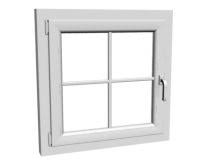
\includegraphics[height=3cm]{images/window.jpg} \\
        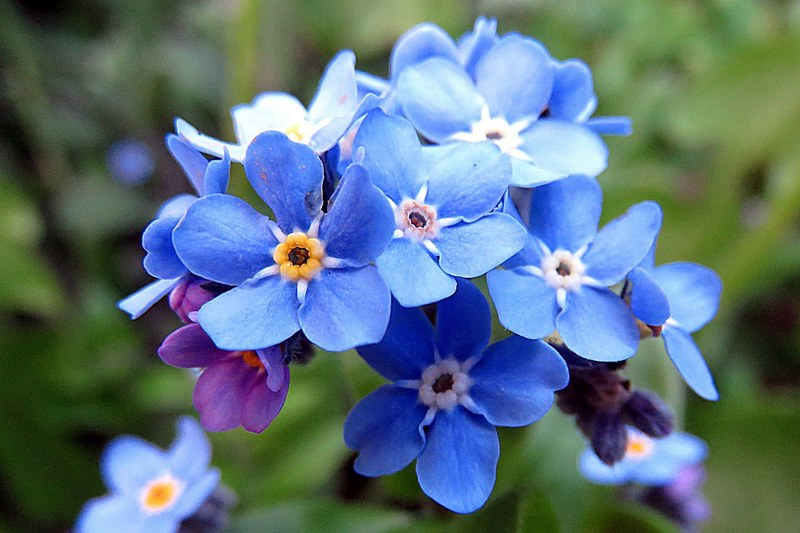
\includegraphics[height=3cm]{images/nezabudka_1.jpg} & 
        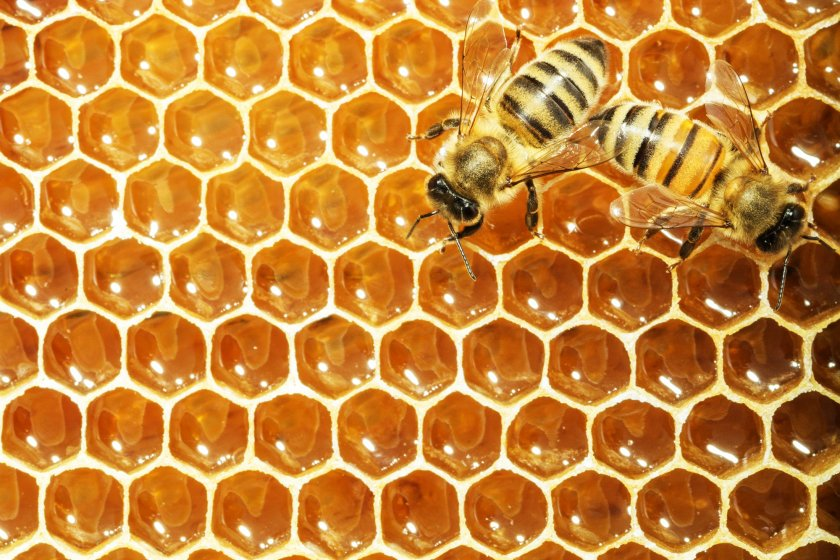
\includegraphics[height=3cm]{images/38018.pkfy9c.840.jpg}
    \end{tabular}
    \caption{Другие объектые, обладающие группами $D_3$, $D_4$, $D_5$ и $D_6$.}
\end{figure}

\subsection{Группа тетраэдра}
%TODO: вот тут мочно нужно будет наприсовать.

Как и в случае с треугольником воспользуемся схожей леммой. Тогда любое движение пространства, сохраняющее на месте тетраэдр однозначно определяется своим действием на вершины. Тем самым, полная группа тетраэдра изоморфна $S_4$.

Собственная же группа состоит из $4 \cdot 3 = 12$ движений: поворот тетраэдра однозначно задаётся своим действием на вершину, и три ребра которые через нее проходят, и может переводить эту вершину в любую из четырёх вершин, после чего, остается ровно три возможности для совмещения рёбер, сохранющее ориентацию пространства. Полный список всех собственных движений тетраэдра: 
\begin{enumerate}
    \item тождественное преобразование;
    \item $4\cdot 2 = 8$ поворотов на углы $\pm 120^\circ$ вокруг прямых, проходящих через вершину и центр противоположной грани;
    \item 3 поворота на $180^\circ$ вокруг прямых, проходящих через середины противоположных рёбер.
\end{enumerate}

В несобственной группе, помимо этих движений, еще содержется 6 отражений $s_{ij}$ в плокостях, проходящих через серидну ребра $ij$ и ребро $kl$. В группе $S_4$ таким отражениям соотвествуют транспозиции букв $i$ и $j$; повороты на $\pm 120^\circ$ переходят в 3-циклы переставляющие буквы $i,j,k$ по циклу, они представляют собой композиции $s_{ij}s_{jk}$; три вращение на $180^\circ$, представляющие собой одновременную тразсопозицию пары вершин, т.е. $s_{ij}s_{kl}$ перехоят в перестановки: $|12\rangle |34\rangle$, $|13\rangle |24\rangle$, $|14\rangle 23\rangle$.

\begin{practice}
    Убедитесь, что вместе в тождественным преобразованием, эти три поворота образуют группу изоморфную $V_4$.
\end{practice}

Оставшиеся 6 несобственных преобразований тетраэдра соотвествуют 4-циклам $|1234\rangle$, $| 1243 \rangle$, $|1324 \rangle $, $| 1342 \rangle $, $|1423 \rangle $, $| 1432 \rangle$. Они реализуются с помощью поворота на $\pm 90^\circ$ вокруг оси, проходящей через середины противоположных рёбер, с последующим отражением относительно ,,сер-\-пер\-ной`` плоскости этого отрезка.

\subsection{Группа додекаэдра}

% TODO: нарисовать его

Воспользуемся той же самой лемой, что и в случае тетраэдра, для определения порядка собственной группы додекаэдра. Движение додекаэдра однозначно определяется действием на вершину и три ребра, тем самым может переводить вершину в любую из 20, а затем тремя способами совмещать рёбра с сохранением ориентации. Поэтому собственная группа додекаэдра состоит из $20 \cdot 3 = 60$ движений.А именно: \begin{enumerate}
    \item тождественное преобразование;
    \item $6 \cdot 4 = 24$ поворота на углы $\frac{2\pi}{n}, \quad n=1,2,3,4$, вокруг осей, проходящих через середины противоположных граней;
    \item 15 поворотов на $180^\circ$ вокруг осей, проходящих через середины противоположных рёбер.
\end{enumerate}

Полная же группа додекаэдра состоит из $20 \cdot 6 = 120$ движений. Помимио перечисленных, туда входят их композиции с центральной симметрией относительно центра додекаэдра.

\begin{practice}
    Проверьте, что полные и собственные группа куба, октаэдра и икосаэдра, соотвественно состоят из 48 и 24, 48 и 24, и 120 и 60 движений.
\end{practice}

% --------------    3
\section{Действие группы на множестве}
\begin{definition}
    [Гомоморфизм групп]
    Отображение $\varphi\colon G_1 \to G_2$ называется \emph{гомоморфизмом}, если переводит композицию в композицию, иначе говоря для любых $a,b \in G_1$ в группе $G_2$ выполняется соотношене \(\varphi(ab) = \varphi(a)\varphi(b)\).

    \emph{Эпиморфизмом} называют сюръективный гомоморфизм, \emph{мономорфизмом} называют инъективный гомоморфизм, а \emph{изоморфизмом}, на самом деле, называют биективный гомоморфизм.
\end{definition}

\begin{practice}
    Докажите, что композиция двух гомоморфизмов --- тоже гомоморфизм.
\end{practice}

\begin{definition}
    [Образ гомоморфизма]
    Множество всех значений гомоморфизма $\varphi \colon G_1 \to G_2$ называется его \emph{образом} и обозначается $\im \varphi$ или $$\varphi (G_1) = \{\varphi(g_1)\mid g_1 \in G_1\}.$$
\end{definition}

\begin{definition}
    [Слой отображения]
    Подмножество $f^{-1}(y) \subset X$ называется \emph{слоем отображения} $f \colon X \to Y$ над точкой $y \in Y$.
\end{definition}

Гомоморфизм переводит единицу в единицу, а обратный в обратный. Докажем только первое. \(\varphi(e_1)\varphi(e_1) = \varphi(e_1e_1)=\varphi(e_1)\), домножая на единицу равенство получаем то, что надо. Отсюда следует, что образ гомоморфизма --- подгруппа. \[\im \varphi \defeq \varphi(G_1) \subset G_2.\]

Напомню, что $\Aut(X)$, где $X$ --- множество, называется множество взаимнооднозначных отображений $X$ в себя, т.е. его перестановки.

\begin{definition}
    [Действие группы на множестве]
Гомоморфизм $\varphi\colon G \to \Aut(X)$ называется \emph{Действием} группы $G$ на множестве $X$ или \emph{представлением} группа $G$ автоморфизмами множества $X$. 

Отображение $\varphi(g) \colon X \to X$, отвечающее элементу $g$ при действии $\varphi$ удобно будет обозначать $\varphi_g \colon X \to X$. Тот факт, что $g \mapsto \varphi_g$ является гомоморфизмом групп означает, что $\varphi_{ab} = \varphi_a \circ \varphi_b$. Если хочется указать, что группа действует на множестве, то пишут $G \colon X$.
\end{definition}

Можно классифицировать действия по разному, приведу в пример классическую. Действие называется \emph{транзитивным}, если любую точку множества $X$ можно перевести в любую другую элементов из $G$. Действие называется \emph{свободным}, если каждое преобразование из $G$ действует на $X$ без неподвижных точек, т.е. $gx = x$ возможно лишь если $g = e$. Действие называется \emph{точным} или \emph{эффектиным}, если любое нетождественное преобразование из $G$ действует не тождественно, т.е. двигает что-то куда-то.

Разберём конкретные примеры действий группы, в первую очередь на себе.
\begin{example}
    [Регулярное действие]
    Пусть $X$ --- множество элементов группы $G$. Тогда \emph{левым регулярным дейсвтиям} называется гомоморфизм $\lambda_g: x \mapsto gx$, для выбраного элемента $g \in G$. Это действительно гомоморфизм групп: \[
        \lambda_{ab}(x) = abx = \lambda_a (bx) = \lambda_a \lambda_b (x).
    \]
    Так как равенство $gx = x$ в группе выполняется только при $g = e$, то такое действие свободно и в частности, эффективно.
    
    \emph{Правым регулярным действием} называется гомоморфизм $\rho_g: x \mapsto xg^{-1}$ правого умножения на обратный.\footnote{Тут $g^{-1}$, конечно, не с проста. Проверьте, что если бы было просто $g$, то преобразование было бы антигомоморфизмом.}

\end{example}
\begin{practice}
    Убедитесь, что $\rho_g$ свободное действие.
\end{practice}

Тем самым, любая абстрактная группа $G$ может быть реализована как группа преобразований некоторого множества. Например, левые регулярные представления числовых групп реализуют аддитивную группу $\R$ группой сдвигов $\lambda_v \colon x \mapsto x + v$ числовой прямой , а мультипликативную группу $\R^\times$ --- группой гомотетий $\lambda_c \colon x \mapsto cx$ проколотой прямой $\R^times = \R \setminus \{0\}$.

\begin{example}
    [Присоединённое действие]
    Отображение $Ad \colon G \to \Aut(G)$, сопоставляющее элементу $g\in G$ автоморфизм сопряжения этим элементом \[Ad_g \colon G \to G, \quad h \mapsto ghg^{-1},\] называется \emph{присоединённым} действием $G$ на себе.


    Образ присоединённого действия $\im Ad$ называется группой \emph{внутренних} автоморфизмов группы $G$ и обозначается $\Int(G)$. Автоморфизмы, которые не лежат в $\Int(G)$, называются, логично, \emph{внешними} автоморфизмами группы $G$. В отличие от левого и правого регулярных действий присоединённое действие, вообще говоря, не свободно и не точно. Заметим также, что если выполняется равенство $h = ghg^{-1}$, то выполняется и равенство $gh = hg$. Подгруппа элементов, которая удовлетворяет такому равенству называется \emph{центром} группы и обозначается \[Z(G) = \{g \in G \mid \forall hj \in G\; gh=hg\}.\]
\end{example}
\begin{practice}
    Убедитесь, что $Ad_g$ является гомоморфизмом, а также и $Ad$.
\end{practice}

\subsection{Орбита и стабилизатор}
Со всякой группой преобразований $G$ множества $X$ связано отношение $x \sim y$ на $X$, означающее, что $y = gx$ для некоторого преобразование $g \in G$. Проверим некоторые важные свойства этого отношения: \begin{conditions} \item \emph{рефлексивность:} $x = ex \implies x \sim x$;
    \item \emph{симметричность:} $y = gx \implies x = g^{-1}y$;
    \item \emph{транзитивность:} $y = gx,\quad z = hy \implies z = ghy$.
\end{conditions}

Такие отношения называются отношениями \emph{эквивалентности}, действительно, логично считать, что точки которые, совмещаются преобразованием из $G$ в каком-то смысле эквиваленты. \emph{Классом эквивалентсости} точки $X$ называются все точки, которые ей эквиваленты. 
\begin{definition}[Орбита]
    Классом эквивалентности отношения $x \sim y \iff gx = y$ называется \emph{орбитой} точки $x$ под действием $G$ и обозначается 
    \[Gx = \{gx \mid g \in G\}.\]

    Множеством всех орбит называется \emph{фактором} множества $X$ под действием $G$ и обозначается $X/G$.
\end{definition}

\begin{proposition}
    Множество $X$ распадается в объединение орбит, в том смысле, что две орбиты либо полностью совпадают, либо вообще не пересекаются. 
\end{proposition}
\begin{proof}
    В самом деле, возьмём две орбиты $Gx$ и $Gy$, а также $z$, который принадлежит и первой и второй орбите: \[g_1x = z, \quad g_2y = z.\]
    В таком случае, устанавливаем, что $$g_1x = g_2y \implies x = g_1^{-1}g_2y \implies y \in G_x.$$
    Тем самым $G_y \subset G_x$, аналогично $G_x \subset G_y$.
\end{proof}

С каждой точкой $x \in X$ и его орбитой $Gx$ связано сюръективное отображение $\ev_x \colon G \twoheadrightarrow Gx,\; g \mapsto gx$, слой которого над точкой $y \in Gx$ состоит из всех преобразований группы $G$, переводящих $x$ в $y$. 
\begin{definition}
    [Транспортёр]
    Слой отображения $\ev_x \colon G \twoheadrightarrow Gx$ над точкой $y$ называется \emph{трансортёром} $x$ в $y$ и обозначается \[G_{xy} = \{g \in G \mid gx = y\}.\]
\end{definition}
\begin{definition}[Стабилизатор]
    Слоем отображения $\ev_x \colon G \twoheadrightarrow Gx$ над самой точкой $x$ называется \emph{стабилизатором} точки $x \in X$ и обозначается \[ \Stab(x) = \{g \in G \mid gx = x \} = G_{xx}.\]
\end{definition}

\begin{lemma}\label{lem:orb_trans}
    Для любых $x, y, z$ из одной орбиты имеются взаимнообратные биекции:
    \begin{center}
        \begin{tikzcd}[column sep = large]
            \Stab(x) \arrow[bend left]{r}{s\mapsto hsg^{-1}} & G_{yz} \arrow[bend left]{l}{f \mapsto h^{-1}fg}
        \end{tikzcd}
    \end{center}
\end{lemma}
\begin{proof}
    Если $y = gx$ и $z = hx$, то $$sg^{-1}y = \underbrace{sx}_{x} = h^{-1}z \implies hsg^{-1} \in G_{yz}, $$
    для всех $s \in \Stab(x)$. Наоборот, если $fy = z$, то \[
        (h^{-1}fg)x = (h^{-1}f)y = {h^{-1}}z = x \implies h^{-1}fg \in \Stab(x).
    \]
\end{proof}

\begin{proposition}
    Стабилизаторы всех точек из одной орбиты равномощны и сопряжены: \[
    y = gx \implies \Stab(y) = g \Stab(x) g^{-1} = \{ ghg^{-1} \mid h \in \Stab(y) \}.\]
    \begin{proof}
        По \cref{lem:orb_trans}, если $z = y$, а $h=g$, следует это утверждение.
    \end{proof}
\end{proposition}
\subsubsection{Связь между орбитой и стабилизатором}

\begin{proposition}[Формула для длины орбиты]
Длина орбиты произвольной точки $x \in X$ при действии на неё конечной группы преобразований $G$ равна $$|Gx| = \frac{|G|}{|\Stab(x)}.$$ В частности, длины всех орбит и порядки стабилизаторов всех точек являются делителем порядка группы.
\end{proposition}
\begin{proof}
    Группа $G$ является объединением непересекающихся множеств $G_{yx}$ по всем $y \in Gx$. Тогда по \cref{lem:orb_trans} все эти множества состоят из $|\Stab(x)|$ элементов. Получаем, что $|Gx|\cdot|\Stab(x)|=|G|.$
\end{proof}



% --------------    4
\subsection{Подсчёт орбит}
Подсчёт числа элементов в факторе $X/G$ (числа орбит) конечного множества $X$ под действием конечной группы $G$ наталкивается на очевидную трудность: посколько длины орбит бывают разными, количество орбит ,,разных типов`` придётся считать по отдельности, по ходу дела уточняя, что такое ,,тип орбиты``. С этим нам поможет следующее утверждение. 
\begin{theorem}[Формула Пойа-Бернсайда]\label{th:burnside}
    Пусть конечная группа $G$ действует на конечном множестве $X$. Для каждого $g \in G$ обозначим, через $X^g = \{x \in X \mid gx = x\} = \{x \in X \mid g \in \Stab(x)\}$ множество неподвижных точек преобразования $g$. Тогда верная следующая формула \[
        |X/G| = \frac{1}{|G|}\cdot \sum_{g \in G} |X^g|.
    \]
\end{theorem}
\begin{proof}
    Обозначим через $F \subset G \times X$ таких пар, что $gx = x$. Такое множество можно описать двумя способами: 
    \[
        F = \bigsqcup_{g\in G} X^g = \bigsqcup_{x \in X} \Stab(x).
    \]
    Первое получается рассмотрением проекции $F \twoheadrightarrow G, (g, x) \mapsto g$: слой над точкой $g$ и есть $^g$. Второе получается проекцией $F \twoheadrightarrow X, (g, x)\mapsto x$: слой над точкой $x$ суть $\Stab(x)$. Согласно первому описанию $|F| = \sum_{g \in G} |X^g|$, а по второму $|F| = \sum_{x \in X} |\Stab(x)| = |G| \cdot |X/G|.$
\end{proof}

\begin{example}[Ожерелья]
    Задача ,,ожерелья`` является одной из классических задач теории групп, действия группы на множестве. На её примере рассмотрим применение формулы \emph{Пойа-Бернсайда}. Эта проблема формулируется обычно как-то так: \emph{<<У~одного очень хитрого мужчины, мистера А.~Л.~Г., есть неограниченный запас бусинок из $n$ цветов. Он хочет подарить как можно большему числу дам подарки-ожерелья из 6 бусин. Дамы заподозрят обман, если поймают мужчину на одинаковых ожерельях. Скольким дамам сможет сделать подарок мистер А.~Л.~Г.?>>}

    Ответом на данный вопрос, конечно же, является количество орбит группы диэдра $D_6$ на множестве всех раскрасок вершин правильно шестиугольника в $n$ цветов. А вы как думали!?

    Группа диэдра $D_6$ состоит из $12$ элементов: \begin{bullets}
        \item тождественного преобразования $e$; 
        \item двух поворотов $r^{\pm 1}$ на $\pm 60^\circ$;
        \item двух поворотов $r^{\pm 2}$ на $\pm 120^\circ$;
        \item центральной симметрии $r^3$;
        \item трёх отражений $s_{14}, s_{25}, s_{36}$ относительно больших диагоналей;
        \item и трёх отражений $\bar{s_{14}}, \bar{s_{25}}, \bar{s_{36}}$ относительно серединных перпендикуляров к сторонам.
    \end{bullets}
    Единица оставляет на месте все $n^6$ раскрасок. Раскраски, симметричные относительно других преобразований, показанных на  рисунке.
    Взяв на этих рисунках все допустимые сочетания цветов, получаем, соотвественно, $n, n^2, n^3, n^4$ и $n^3$ раскрасок. Тогда по \cref{th:burnside} число 6-бусинок равно \[\frac{n^6 + 3n^4 +4n^3+2n^2+2n}{12}.\]

\end{example}
    \begin{figure}[ht]
        \centering
        \begin{asy}
            size(4.5cm);
            currentpen=fontsize(10);
            circle omega = circle(origin(), 2); draw(omega);
            point A = angpoint(omega, 30);
            point B = angpoint(omega, 90);
            point C = angpoint(omega, 150);
            point D = angpoint(omega, 210);
            point E = angpoint(omega, 270);
            point F = angpoint(omega, 330);

            draw(A--D, blue);
            draw(B--E, blue);
            draw(C--F, blue);

            dot(A, invisible+1,  filltype=FillDraw(fillpen=blue+white, drawpen=blue));
            dot(B, invisible+1,  filltype=FillDraw(fillpen=blue+white, drawpen=blue));
            dot(C, invisible+1,  filltype=FillDraw(fillpen=blue+white, drawpen=blue));
            dot(D, invisible+1,  filltype=FillDraw(fillpen=blue+white, drawpen=blue));
            dot(E, invisible+1,  filltype=FillDraw(fillpen=blue+white, drawpen=blue));
            dot(F, invisible+1,  filltype=FillDraw(fillpen=blue+white, drawpen=blue));


            label("1", B, dir(90)*1.5);
            label("2", C, dir(150)*1.5);
            label("3", D, dir(210)*1.5);
            label("4", E, dir(270)*1.5);
            label("5", F, dir(330)*1.5);
            label("6", A, dir(30)*1.5);

            draw(arc(circle(origin(), 0.9), 30, 90), red, Arrow);

            label("$r$-инвариантные бусы", (0, -3));
        \end{asy}
        \qquad
        \begin{asy}
            size(4.5cm);
            currentpen=fontsize(10);
            point O = (0, 0);
            circle omega = circle(O, 2); draw(omega);
            point A = angpoint(omega, 30);
            point B = angpoint(omega, 90);
            point C = angpoint(omega, 150);
            point D = angpoint(omega, 210);
            point E = angpoint(omega, 270);
            point F = angpoint(omega, 330);

            draw(A--O, red);
            draw(B--O, blue);
            draw(C--O, red);
            draw(D--O, blue);
            draw(E--O, red);
            draw(F--O, blue);

            dot(A, invisible+1,  filltype=FillDraw(fillpen=red+white, drawpen=red));
            dot(B, invisible+1,  filltype=FillDraw(fillpen=blue+white, drawpen=blue));
            dot(C, invisible+1,  filltype=FillDraw(fillpen=red+white, drawpen=red));
            dot(D, invisible+1,  filltype=FillDraw(fillpen=blue+white, drawpen=blue));
            dot(E, invisible+1,  filltype=FillDraw(fillpen=red+white, drawpen=red));
            dot(F, invisible+1,  filltype=FillDraw(fillpen=blue+white, drawpen=blue));


            label("1", B, dir(90)*1.5);
            label("2", C, dir(150)*1.5);
            label("3", D, dir(210)*1.5);
            label("4", E, dir(270)*1.5);
            label("5", F, dir(330)*1.5);
            label("6", A, dir(30)*1.5);

            draw(arc(circle(origin(), 0.9), -30, 90), red, Arrow);

            label("$r^2$-инвариантные бусы", (0, -3));
        \end{asy}
        \qquad
        \begin{asy}
            size(4.5cm);
            currentpen=fontsize(10);
            point O = (0, 0);
            circle omega = circle(O, 2); draw(omega);
            point A = angpoint(omega, 30);
            point B = angpoint(omega, 90);
            point C = angpoint(omega, 150);
            point D = angpoint(omega, 210);
            point E = angpoint(omega, 270);
            point F = angpoint(omega, 330);

            draw(O--A, red, Arrow);
            draw(O--B, blue, Arrow);
            draw(O--C, deepgreen, Arrow);
            draw(O--D, red, Arrow);
            draw(O--E, blue, Arrow);
            draw(O--F, deepgreen, Arrow);

            dot(A, invisible+1,  filltype=FillDraw(fillpen=red+white, drawpen=red));
            dot(B, invisible+1,  filltype=FillDraw(fillpen=blue+white, drawpen=blue));
            dot(C, invisible+1,  filltype=FillDraw(fillpen=deepgreen+white, drawpen=deepgreen));
            dot(D, invisible+1,  filltype=FillDraw(fillpen=red+white, drawpen=red));
            dot(E, invisible+1,  filltype=FillDraw(fillpen=blue+white, drawpen=blue));
            dot(F, invisible+1,  filltype=FillDraw(fillpen=deepgreen+white, drawpen=deepgreen));


            label("1", B, dir(90)*1.5);
            label("2", C, dir(150)*1.5);
            label("3", D, dir(210)*1.5);
            label("4", E, dir(270)*1.5);
            label("5", F, dir(330)*1.5);
            label("6", A, dir(30)*1.5);

            label("$r^3$-инвариантные бусы", (0, -3));
        \end{asy}

        \begin{asy}
            size(4.5cm);
            currentpen=fontsize(10);
            point O = (0, 0);
            circle omega = circle(O, 2); draw(omega);
            point A = angpoint(omega, 30);
            point B = angpoint(omega, 90);
            point C = angpoint(omega, 150);
            point D = angpoint(omega, 210);
            point E = angpoint(omega, 270);
            point F = angpoint(omega, 330);

            draw(C--F, deepgreen+dashed);
            draw(0.5*B + 0.5*D -- B, red, Arrow);
            draw(0.5*B + 0.5*D -- D, red, Arrow);
            draw(0.5*A + 0.5*E -- A, blue, Arrow);
            draw(0.5*A + 0.5*E -- E, blue, Arrow);

            dot(A, invisible+1,  filltype=FillDraw(fillpen=blue+white, drawpen=blue));
            dot(B, invisible+1,  filltype=FillDraw(fillpen=red+white, drawpen=red));
            dot(C, invisible+1,  filltype=FillDraw(fillpen=deepgreen+white, drawpen=deepgreen));
            dot(D, invisible+1,  filltype=FillDraw(fillpen=red+white, drawpen=red));
            dot(E, invisible+1,  filltype=FillDraw(fillpen=blue+white, drawpen=blue));
            dot(F, invisible+1,  filltype=FillDraw(fillpen=deepgreen+white, drawpen=deepgreen));


            label("1", B, dir(90)*1.5);
            label("2", C, dir(150)*1.5);
            label("3", D, dir(210)*1.5);
            label("4", E, dir(270)*1.5);
            label("5", F, dir(330)*1.5);
            label("6", A, dir(30)*1.5);

            label("$s_{25}$-инвариантные бусы", (0, -3));
        \end{asy}
        \qquad
        \begin{asy}
            size(4.5cm);
            currentpen=fontsize(10);
            point O = (0, 0);
            circle omega = circle(O, 2); draw(omega);
            point A = angpoint(omega, 30);
            point B = angpoint(omega, 90);
            point C = angpoint(omega, 150);
            point D = angpoint(omega, 210);
            point E = angpoint(omega, 270);
            point F = angpoint(omega, 330);

            point A1 = angpoint(omega, 120);
            point D1 = angpoint(omega, 300);

            draw(A1--D1, orange+dashed);
            draw(0.5*B + 0.5*C -- B, red, Arrow);
            draw(0.5*B + 0.5*C -- C, red, Arrow);
            draw(0.5*E + 0.5*F -- E, blue, Arrow);
            draw(0.5*E + 0.5*F -- F, blue, Arrow);
            draw(0.5*A + 0.5*D -- A, deepgreen, Arrow);
            draw(0.5*A + 0.5*D -- D, deepgreen, Arrow);

            dot(A, invisible+1,  filltype=FillDraw(fillpen=deepgreen+white, drawpen=deepgreen));
            dot(B, invisible+1,  filltype=FillDraw(fillpen=red+white, drawpen=red));
            dot(C, invisible+1,  filltype=FillDraw(fillpen=red+white, drawpen=red));
            dot(D, invisible+1,  filltype=FillDraw(fillpen=deepgreen+white, drawpen=deepgreen));
            dot(E, invisible+1,  filltype=FillDraw(fillpen=blue+white, drawpen=blue));
            dot(F, invisible+1,  filltype=FillDraw(fillpen=blue+white, drawpen=blue));


            label("1", B, dir(90)*1.5);
            label("2", C, dir(150)*1.5);
            label("3", D, dir(210)*1.5);
            label("4", E, dir(270)*1.5);
            label("5", F, dir(330)*1.5);
            label("6", A, dir(30)*1.5);

            label("$\bar{s_{36}}$-инвариантные бусы", (0, -3));
        \end{asy}

        \caption{Симметричные ожерелья из 6 бусин.}
    \end{figure}


% --------------    5
\section{Кольцо многочленов}
\subsection{Деление с остатком} 

\subsection{Неприводимые многочлены}
\subsection{Теорема Безу}
\subsection{Факториальность кольца}

% --------------    6
\section{Комплексные числа}
\subsection{Первообразные корни и круговые многочлены}

% --------------    7
\subsection{Гауcсовы числа}
\subsubsection{Пифогоровы тройки}
\subsubsection{Теорема Ферма-Эйлера-Гаусса}


\newpage
\renewcommand{\thesubsection}{\roman{subsection}}
\setcounter{subsection}{0}

\section*{Задачи}
\addcontentsline{toc}{section}{Задачи}

% TODO: Сделать "словарик" в задачах
\subsection{Перестановки}
\begin{enumerate}
    \item Возьмите какое-нибудь четырёхбуквенное слово, скажем, прошлое слово \textsf{УШКА}.
        Покажите, что все варианты (\emph{А сколько, кстати, их?}) тоже разбиваются на две группы,
        и обмен двух букв местами переводит нас из одной группы в другую.
    \item Вова сказал своей подруге, что подарит ей доширак,
        если она в слове \textsf{КОМАНДА} сделает семь попарных обменов и получит исходное слово.
        В чём просчитался Вова?
    \item Найти цикловой тип, порядок и четность перестановки
        \[
            \sigma = \begin{pmatrix}
                1 & 2 & 3 & 4 & 5 & 6 & 7 & 8 & 9 & 10 & 11 \\
                5 & 9 & 1 & 3 & 2 & 11 & 10 & 8 & 4 & 7 & 6
            \end{pmatrix}.
        \]
    \item Найдите все перестановки трехэлементного множества.
    \item Сколько существует перестановок слова \textsf{РЫБА}, состоящих ровно
        из двух циклов? Найдите эти слова.
    \item Докажите, что любая перестановка имеет обратную.
    \item Найдите обратную перестановку для: 

        \begin{enumerate*}[(a), itemjoin=;\qquad]
            \item \(\begin{pmatrix}
                    1 & 2 & 3 & 4 \\
                    2 & 1 & 4 & 3
                \end{pmatrix}\)
            \item \(\begin{pmatrix}
                    1 & 2 & 3 & 4 & 5 \\
                    2 & 1 & 4 & 5 & 3
                \end{pmatrix}\).
        \end{enumerate*} 
    \item Верно ли, что композиция двух циклов длины 2 является перестановкой порядка 1 или 2?
    \item Пусть дана перестановка в виде композиции циклов  \[
            \sigma = | 1, 4, 7 \rangle |2, 5 \rangle
        .\]  
        Напишите ее ``матричный вид'', ее порядок и обратную ей.
    \item Пусть даны две перестановки \[
            \sigma = | 1, 4, 2 \rangle 
            , \quad
            \tau = | 1, 3 \rangle | 2, 5 \rangle
        .\]
        Найдите композиции $\tau \circ \sigma$ и $\sigma \circ \tau$, четность и порядок этих композиций.
        А также их ``матричный вид''.
    \item Пусть даны две перестановки \[
            \sigma = | 1, 8, 5, 2 \rangle | 3, 7 \rangle
            , \quad
            \tau = | 1, 4\rangle |2,  3, 6 \rangle | 5, 8 \rangle
            .
        \]
        Найдите композиции $\tau \circ \sigma$ и $\sigma \circ \tau$, четность и порядок этих композиций.

\end{enumerate}

\subsection{Группы}
\begin{enumerate}
    \item Сколько элементов в группе $D_5$? А сколько элементов порядка $2$?
    \item Докажите, что $A_n$ --- подгруппа группы $S_n$.
    \item Верно ли, что подгруппа абелевой группы всегда абелева? Если да — объясните. Если нет — приведите контрпример.
    \item В группе $D_6$ найдите композицию $r \circ s_1$, где $r$ --- поворот на $60^\circ$, а $s_1$ --- отражение относительно вертикальной оси.
    \item Напишите таблицу Кэли для группы $S_3$. Какие из элементов коммутируют между собой?
    \item Докажите, что в группе $D_n$ выполняется равенство: \[
            s \circ r = r^{-1} \circ s.
        \]
        Где $r$ --- поворот на $\rfrac{360^\circ}{n}$, а $s$ --- отражение относительно любой оси.
    % \item Докажите, что в группе порядка 15 не может быть подгруппы порядка 4.
    % \item Пусть порядок группы равен 12. Докажите, что порядок любой подгруппы делит 12. Может ли в этой группе существовать элемент порядка 7?
    % \item Докажите, что все элементы порядка $2$ и единица в группе $S_n$ образуют подгруппу. 
    \item Пусть $H = (\{-1, 1\}, \times)$ в $(\R^*, \times).$\footnote{Здесь ,,звёздочка`` обозначает то, что нет нуля.} Является ли $H$ подгруппой? Является ли $H$ абелевой?
    \item Изоморфны ли группы
        \begin{inumerate}
        \item $S_2$ и $\Z/(2)$
        \item $S_3$ и $\Z/(3)$
        \item $D_4$ и $S_4$
        \item $S_4$ и $D_{12}$
        \item[(f*)] $S_5$ и $D_{10}$
        \end{inumerate}.
    \item Найдите все подгруппы в 
        \begin{inumerate}
        \item $\Z/(6)$
        \item $S_3$
        \item $D_4$
        \item $D_6$
        \item[(e*)] $D_{12}$
        \item[(f*)] $A_4$
        \end{inumerate}.
    Для каждой подгруппы проверьте, что ее порядок делит порядок всей группы. Подумайте над тем, каким группам изоморфны каждая из них.
\item Летнешкольников заставили выложить плац правильной шестиугольной плиткой\footnote{Причем плитка самая обычная, на ней даже узоров никаких нет.}. Сколько существует симметрий такого замощения плиткой? Образуют ли они группу?
        Если да, то какой у нее порядок?
    \item Пусть $H$ --- множество всех перестановок из $S_4$, которые оставляют
        тройку на месте. Является ли $H$ подгруппой группы $S_3$?
        Если да, то какой у нее порядок и является ли она абелевой?
    \item Является ли множество $G = \{2^n \mid n \in \Z\}$ с операцией умножения группой?
        Если да, то является ли она абелевой? Какие в ней подгруппы?
    \item Придумайте свой объект, например, букву ,,Ж``. Опишите его группу симметрий. Подумайте, какой группе она изоморфна.
    \item Пусть $H$ подгруппа группы $G$. Тогда \emph{левым смежным классом} называется \(gH =\{gh \mid h \in H\}.\)
        \begin{enumerate}[(a)]
        \item Докажите, что два смежных класса либо совпадают, либо не пересекаются.
        \item[(b)*] Докажите, что все смежные классы находятся в биекции друг с другом.
        \addtocounter{enumii}{1}
        \item В каком соотношении находится порядок группы $H$, число смежных классов и порядок группы $G$?
        \item Почему в группе порядка $15$ не может быть подгруппы порядка $4$?
        \end{enumerate}
\end{enumerate}

\subsection{Орбита и стабилизатор. Собственные группы фигур}
\begin{enumerate}
    \item Пусть $\varphi \colon \Z \to \Z/(6)$ гомоморфизм, который $n \mapsto n \pmod 6.$
        \begin{enumerate}
            \item Является ли он изоморфизмом?
            \item Найдите $\ker \varphi.$
            \item Чем являются элементы $\im \varphi$.
        \end{enumerate}
    \item Пусть $H = \{e, |1 2\rangle \}$ подгруппа $S_3$. Постройте гомоморфизм
         $\psi \colon S_3 \to H$, такой что четные перестановки он переводит в  $e.$
         А нечетные в $|1 2 \rangle$. 
         \begin{enumerate}
             \item Проверьте, что гомоморфизм $\psi$ сохраняет композицию.
             \item Найдите $\ker \psi$.
             \item Проверьте, что $S_3/\ker\psi \cong H$.
         \end{enumerate}
     \item Группа $D_4$ действует на множестве вершин квадрата $\{1, 2, 3, 4\}$.
         \begin{enumerate}
             \item Сколько орбит у этого действия?
             \item Найдите стабилизатор вершины 1.
             \item Проверьте, что \(
             |D_4| = |\Stab(1)| \cdot |\Orb(1)|
             .\)
         \end{enumerate}
     \item Группа $S_3$ действует на многочлене $P(x_1, x_2, x_3) = x_1x_2 + x_2x_3$,
         переставляя переменные. Найдите орбиты этого действия. Какой стабилизатор у $P$?
     \item Пусть задан гомоморфизм $\mu \colon \Z/(12) \to \Z/(12)$, который $z \mapsto 3z$.
         \begin{enumerate}
             \item Найдите $\ker \mu$.
             \item Постройте таблицу Кэли для $\im \mu$.
             \item Изоморфна ли $\im \mu$ какой-то известной группе?
         \end{enumerate}

\end{enumerate}
          % TODO: ПЕРЕПИСАТЬ НАХУЙ
\subsection{Лемма Бернсайда и теорема Пойа: ожерелья, орнаменты}
% 

\subsection{Многочлены}
% \begin{enumerate}
    \item Сколькими разными способами можно раскрасить грани тетраэдра в $n$ цветов, где две раскраски считаются \emph{одинаковыми}, если одну можно получить поворотов другой.
    \item Сколькими различными способами можно составить ожерелье из $n$ цветов, в котором будет \begin{enumerate}
        \item 5 бусин;
        \item 6 бусин;
        \item 7 бусин.
    \end{enumerate}

    \item Флаг некоторой страны состоит из трёх горизонтальных полос. Сколькими способами можно раскрасить его в $n$ цветов. Если флаги, отличающиеся перестановкой полос, считаются одинаковыми.

    \item Сколькими разными способами можно раскрасить рёбра куба в $n$ цветов, где две раскраски считаются \emph{одинаковыми}, если одну можно получить поворотов другой.

    \item Сколькими способами можно раскрасить клетки шахматной доски $4 \times 4$ в чёрный и белый цвета, две раскраски считаются одинаковыми: \begin{enumerate}
            \item если одну можно получить из другой поворотом;
            \item если одна получается из другой под действием элемента группы $D_4$.
    \end{enumerate}

    \item Правильный шестиугольник разбит на 6 равносторонних треугольников. Сколькими способами можно раскрасить эти треугольники в 3 цвета, если расраски совпадающие, при повороте на угол $60^\circ$, считаются одинаковыми?

    \item Молекула имеет форму правильного тетраэдра, в каждой вершине которой может находиться один из атомов: $H$ (водород), $Cl$ (хлор), $Br$ (бром). Сколько существует различных молекул, если молекулы, совпадающие при вращении, считаются одинаковыми, но при отражения (зеркальные изомеры) считаются разными?
\end{enumerate}

\subsection{Комплексные числа}
% \input{problems/sixth.tex}
\subsection{Гауссовы числа ,,в хвост и в гриву``} % этого листка не будет на семинарах
% \subsection{problems/seventh.tex}

\newpage
\markboth{Контрольная работа}{Контрольная работа}
\addcontentsline{toc}{section}{Контрольная работа}
\section*{Контрольная работа}
% \input{tasks/exam.tex}

\end{document}


